\documentclass[11pt,a4paper]{article}
\usepackage[utf8]{inputenc}
\usepackage[T1]{fontenc}
\usepackage{lmodern}
\usepackage[margin=2cm]{geometry}
\usepackage{amsmath,amssymb}
\usepackage{booktabs}
\usepackage{graphicx}
\usepackage{hyperref}
\usepackage{xcolor}
\usepackage{titlesec}
\usepackage{tabularx}
\usepackage{float}

\hypersetup{
    colorlinks=true,
    linkcolor=blue!70!black,
    citecolor=blue!70!black,
    urlcolor=blue!70!black
}

\titleformat{\section}{\large\bfseries}{\thesection.}{0.5em}{}
\titleformat{\subsection}{\normalsize\bfseries}{\thesubsection.}{0.5em}{}
\titlespacing*{\section}{0pt}{1.2ex plus 0.5ex minus .2ex}{0.6ex}
\titlespacing*{\subsection}{0pt}{1.0ex plus 0.4ex minus .2ex}{0.4ex}

\setlength{\parskip}{0.45em}
\setlength{\parindent}{0pt}

\begin{document}

\begin{center}
    {\LARGE \textbf{Projeto 1: Regressão com MLP e Estudo de Ablação}} \\[0.35em]
    {\large Disciplina: Introdução às Redes Neurais Artificiais} \\[0.3em]
    \textbf{Autor:} Vinícius Augusto Landim Andrade (RA: 169251) \\[0.2em]
    \textbf{Repositório / Código Reprodutível:} \url{https://github.com/vinicius-landim/neural-networks-course/tree/main/mlp/src}
\end{center}
\vspace{-0.5em}
\hrule
\vspace{0.8em}

\section{Configuração Experimental e Reprodutibilidade}

\subsection{Pré-processamento e Partição dos Dados (se necessário)}
A partição dos dados seguiu estritamente a proporção de 10\% para treino, 10\% para validação e 80\% para teste.
Essa restrição intencional no volume de treino torna a tarefa suscetível ao sobreajuste, tornando a investigação de hiperparâmetros e técnicas de regularização crítica. As amostras selecionadas para treino podem ser obsevadas na figura \ref{fig:amostragem}.

\begin{figure}[H]
    \centering
    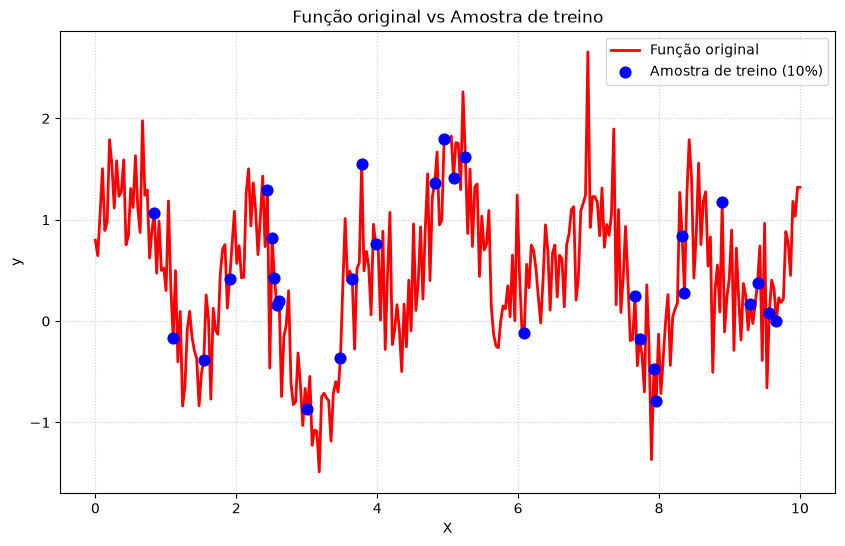
\includegraphics[width=0.6\textwidth]{../data/amostragem.png}
    \caption{Função original vs Amostra de treino}
    \label{fig:amostragem}
\end{figure}

O pré-processamento incluiu a padronização dos atributos por distribuição através do \texttt{StandardScaler} da biblioteca \textit{scikit-learn}. Para assegurar a integridade do experimento e mitigar qualquer vazamento de dados (\textit{data leakage}), o cálculo das médias e desvios-padrão (\textit{fit}) ocorreu exclusivamente sobre as 30 amostras do conjunto de treino. Posteriormente, as métricas de escalonamento foram aplicadas (\textit{transform}) de forma isolada às partições de validação e teste.

\subsection{Definição e Otimização Empírica do Modelo Baseline (Vanilla)}
O modelo \textit{baseline} consiste em uma rede \textit{Multi-Layer Perceptron} (MLP) básica, implementada em PyTorch e treinada estritamente com o algoritmo de otimização SGD (sem aceleradores adaptativos como Adam e com termo de \textit{momentum} igual a 0.0). Nenhuma regularização explícita (L1, L2 ou Dropout) foi aplicada nesta fase inicial, estabelecendo um ponto de partida puramente não-regularizado.

A busca empírica pela melhor configuração baseou-se na variação da profundidade da rede e na largura das camadas densas. Vale ressaltar que as escolhas para o Modelo Baseline foram feitas avaliando os resultados para treino e validação, sendo o conjunto de teste verificado somente após a definição da arquitetura.

A topologia final selecionada para o baseline (e mantida para os estudos de ablação) é composta por três camadas ocultas com 64, 128 e 64 neurônios, respectivamente, intercaladas por funções de ativação ReLU. O treinamento utilizou \textit{mini-batches} de 5 amostras e uma taxa de aprendizado ($\eta$) fixada em 0.01 ao longo de 5.000 épocas. Os melhores pesos foram salvos através de um \textit{checkpoint} do modelo no menor Erro Quadrático Médio (MSE) alcançado no conjunto de validação.

A Tabela~\ref{tab:baseline_hiper} detalha o espaço de hiperparâmetros explorado e a configuração final selecionada.

\begin{table}[h]
\centering
\small
\caption{Espaço amostrado e configuração final da MLP Baseline (Vanilla).}
\label{tab:baseline_hiper}
\begin{tabularx}{\textwidth}{
    >{\raggedright\arraybackslash}p{0.25\textwidth} 
    >{\raggedright\arraybackslash}X 
    >{\raggedright\arraybackslash}p{0.30\textwidth}
}
\toprule
\textbf{Hiperparâmetro} & \textbf{Valores Explorados} & \textbf{Configuração Escolhida (Vanilla)} \\
\midrule
Topologia das Camadas & 1, 2 e 3 camadas ocultas; 16, 32, 64 e 128 neurônios & Entrada $\rightarrow$ 64 $\rightarrow$ 128 $\rightarrow$ 64 $\rightarrow$ Saída \\
\addlinespace
Função de Ativação & ReLU, Tanh & ReLU \\
\addlinespace
Otimizador & SGD puro (sem \textit{momentum}) & SGD ($\eta = 0.01$) \\
\addlinespace
Tamanho do Lote (\textit{Batch Size}) & 5, 10, 30 amostras & 5 \\
\addlinespace
Função de Custo & Erro Quadrático Médio (MSE) & MSE  \\
\addlinespace
Treinamento e Seleção & 5.000 épocas; monitoramento pelo menor MSE de validação & 5.000 épocas (resgate do melhor \textit{checkpoint}) \\
\addlinespace
Semente Aleatória & Sementes fixas para reprodutibilidade & \texttt{seed = 42} \\
\bottomrule
\end{tabularx}
\end{table}
\vspace{1em}

O modelo \textit{Vanilla} atingiu seu ponto ótimo de convergência na época 2422. As métricas registradas neste \textit{checkpoint} foram:

\begin{itemize}
    \item \textbf{Métricas no Treinamento:} MSE = $0.1007$, RMSE = $0.3173$ e MAE = $0.2444$
    \item \textbf{Métricas na Validação:} MSE = $0.3046$, RMSE = $0.5519$ e MAE = $0.4420$
\end{itemize}

Observe a existência de uma discrepância entre os erros, com o MSE de validação sendo aproximadamente três vezes maior que o de treinamento. Isso representa um caso de \textit{overfitting}, sendo esse comportamento esperado dado o tamanho restrito dos dados de treino e a arquitetura definida.

\section{Dinâmica de Treinamento e Convergência (Baseline vs. Modificados)}

A evolução das curvas de função de perda (MSE) e da métrica auxiliar (MAE) ao longo das épocas foi monitorada para verificar a estabilidade do otimizador e comparar a dinâmica do \textit{baseline} com os modelos submetidos ao estudo de ablação. As figuras \ref{fig:loss_baseline}, \ref{fig:loss_momentum}, \ref{fig:loss_l2}, \ref{fig:loss_l1} e \ref{fig:loss_dropout} ilustram essas trajetórias.

\begin{figure}[H]
    \centering
    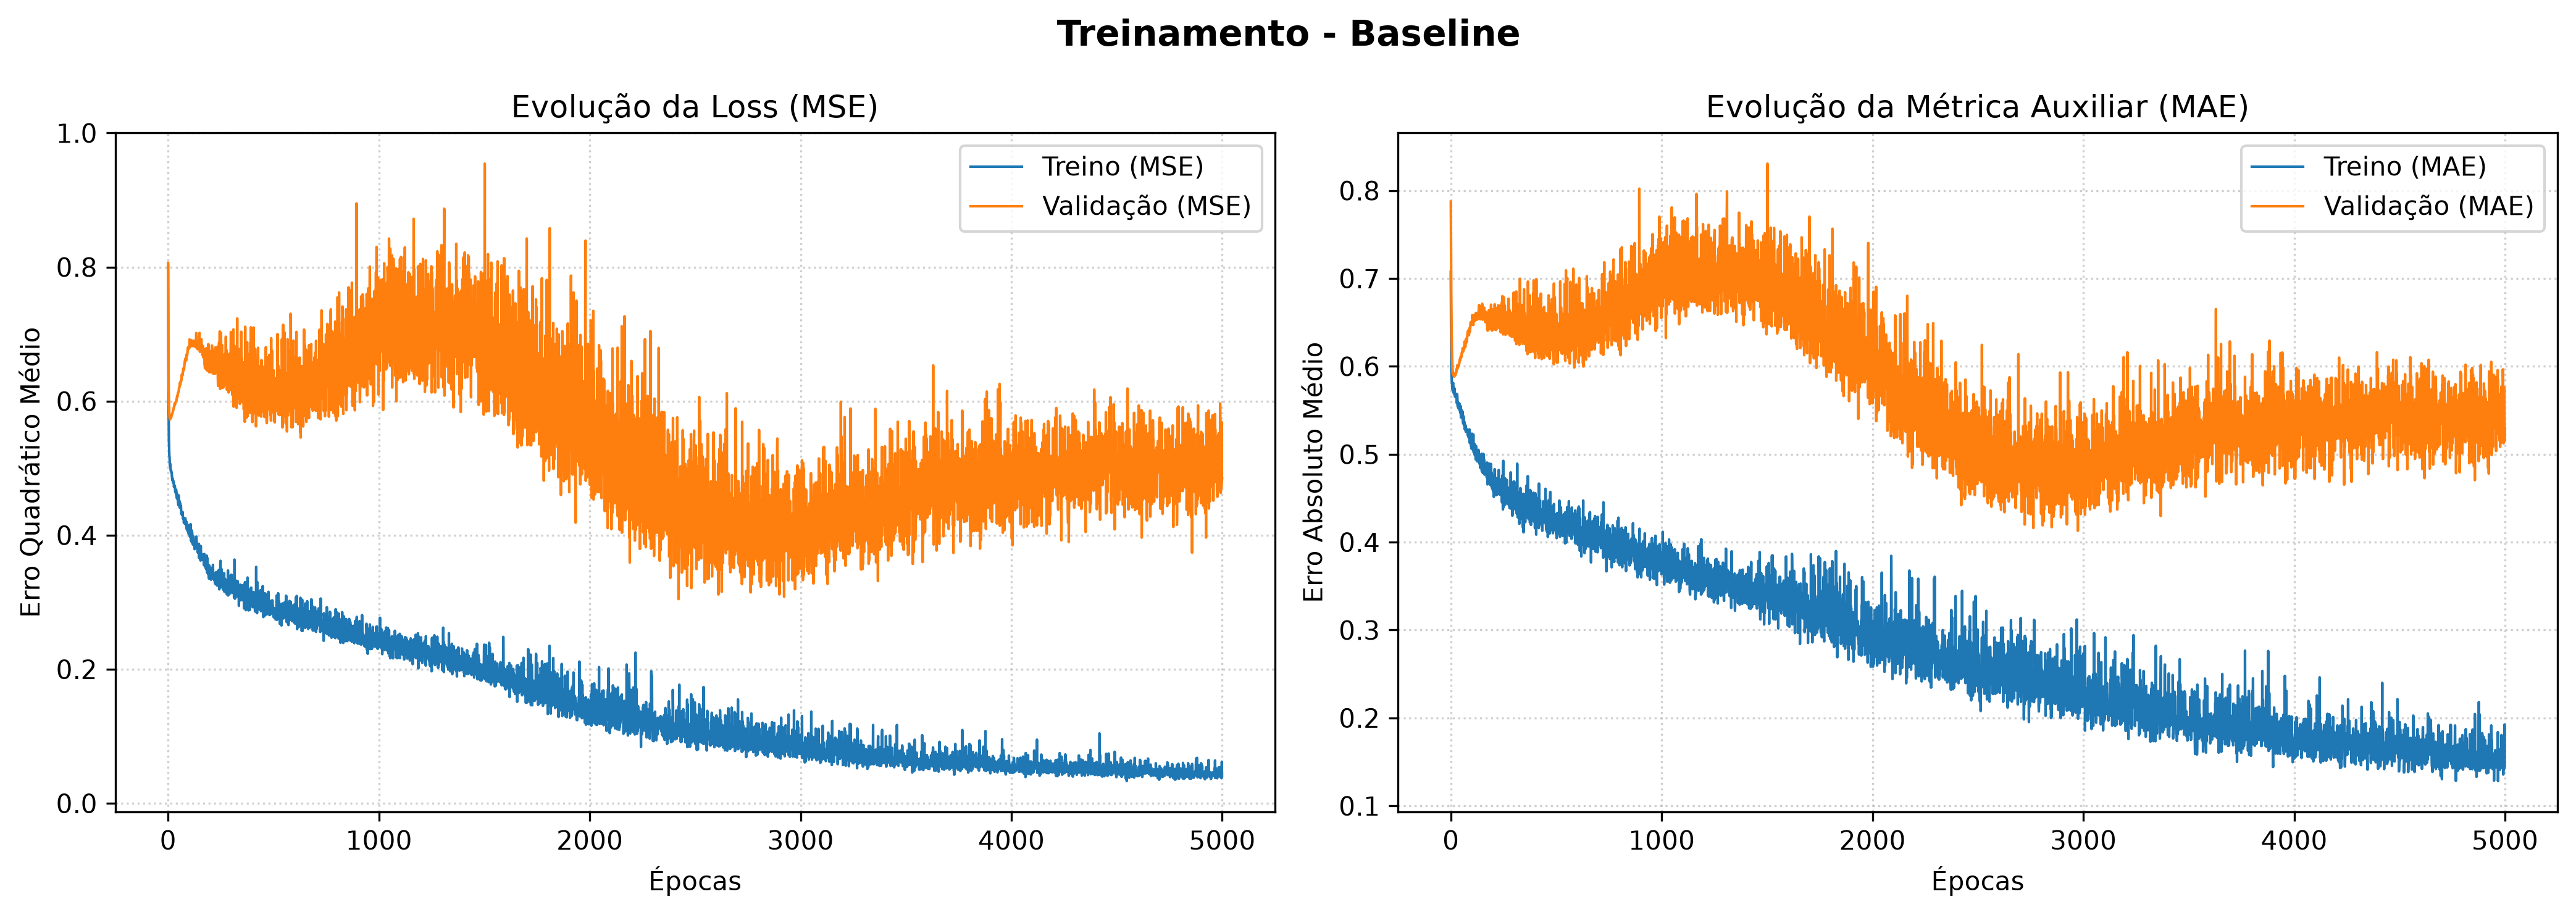
\includegraphics[width=\textwidth]{../src/outputs/baseline_history.png}
    \caption{Convergência da MLP Baseline (Vanilla).}
    \label{fig:loss_baseline}
\end{figure}

\begin{figure}[H]
    \centering
    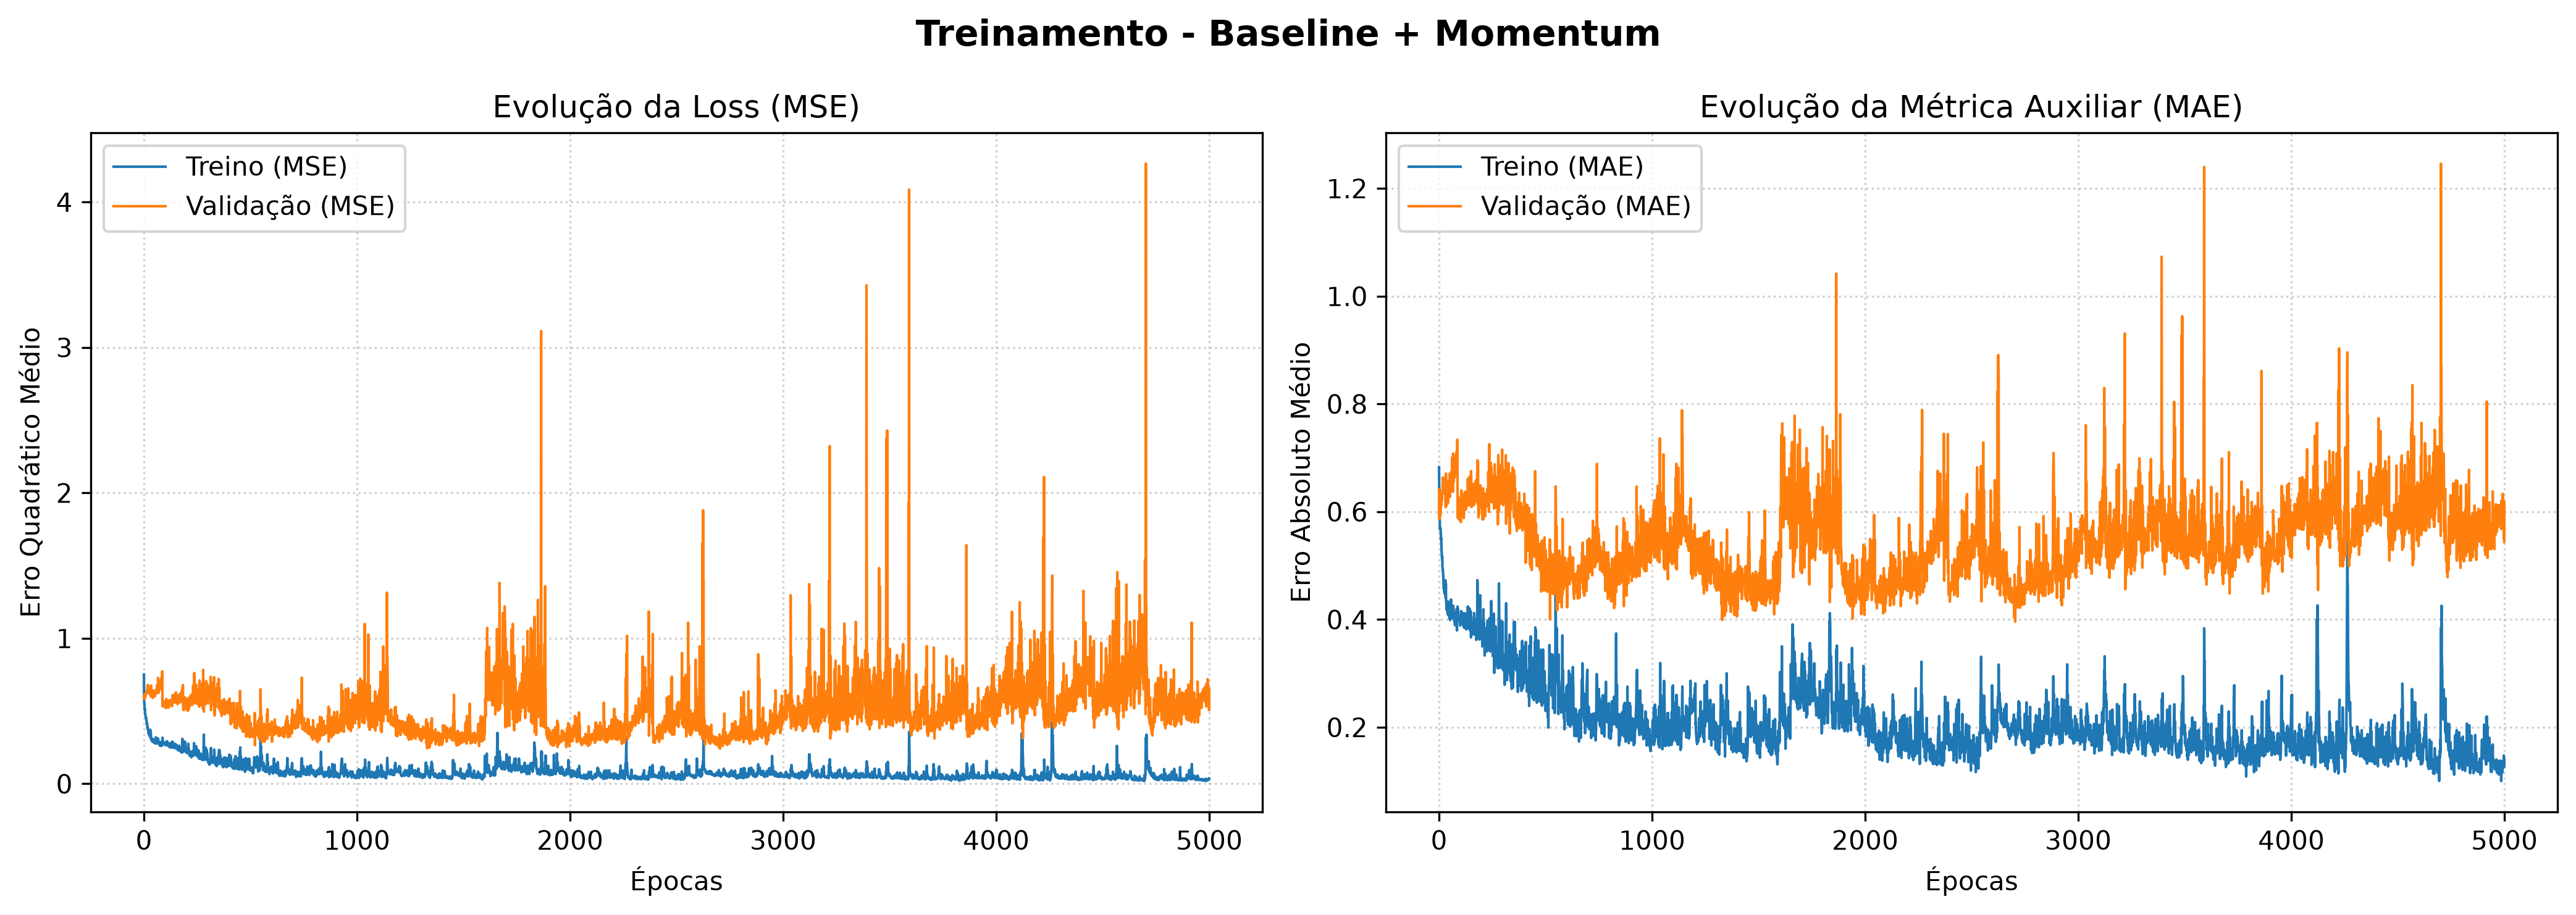
\includegraphics[width=\textwidth]{../src/outputs/baseline_e_momentum_history.png}
    \caption{Convergência da MLP Baseline com Momentum ($\beta=0.9$).}
    \label{fig:loss_momentum}
\end{figure}

\begin{figure}[H]
    \centering
    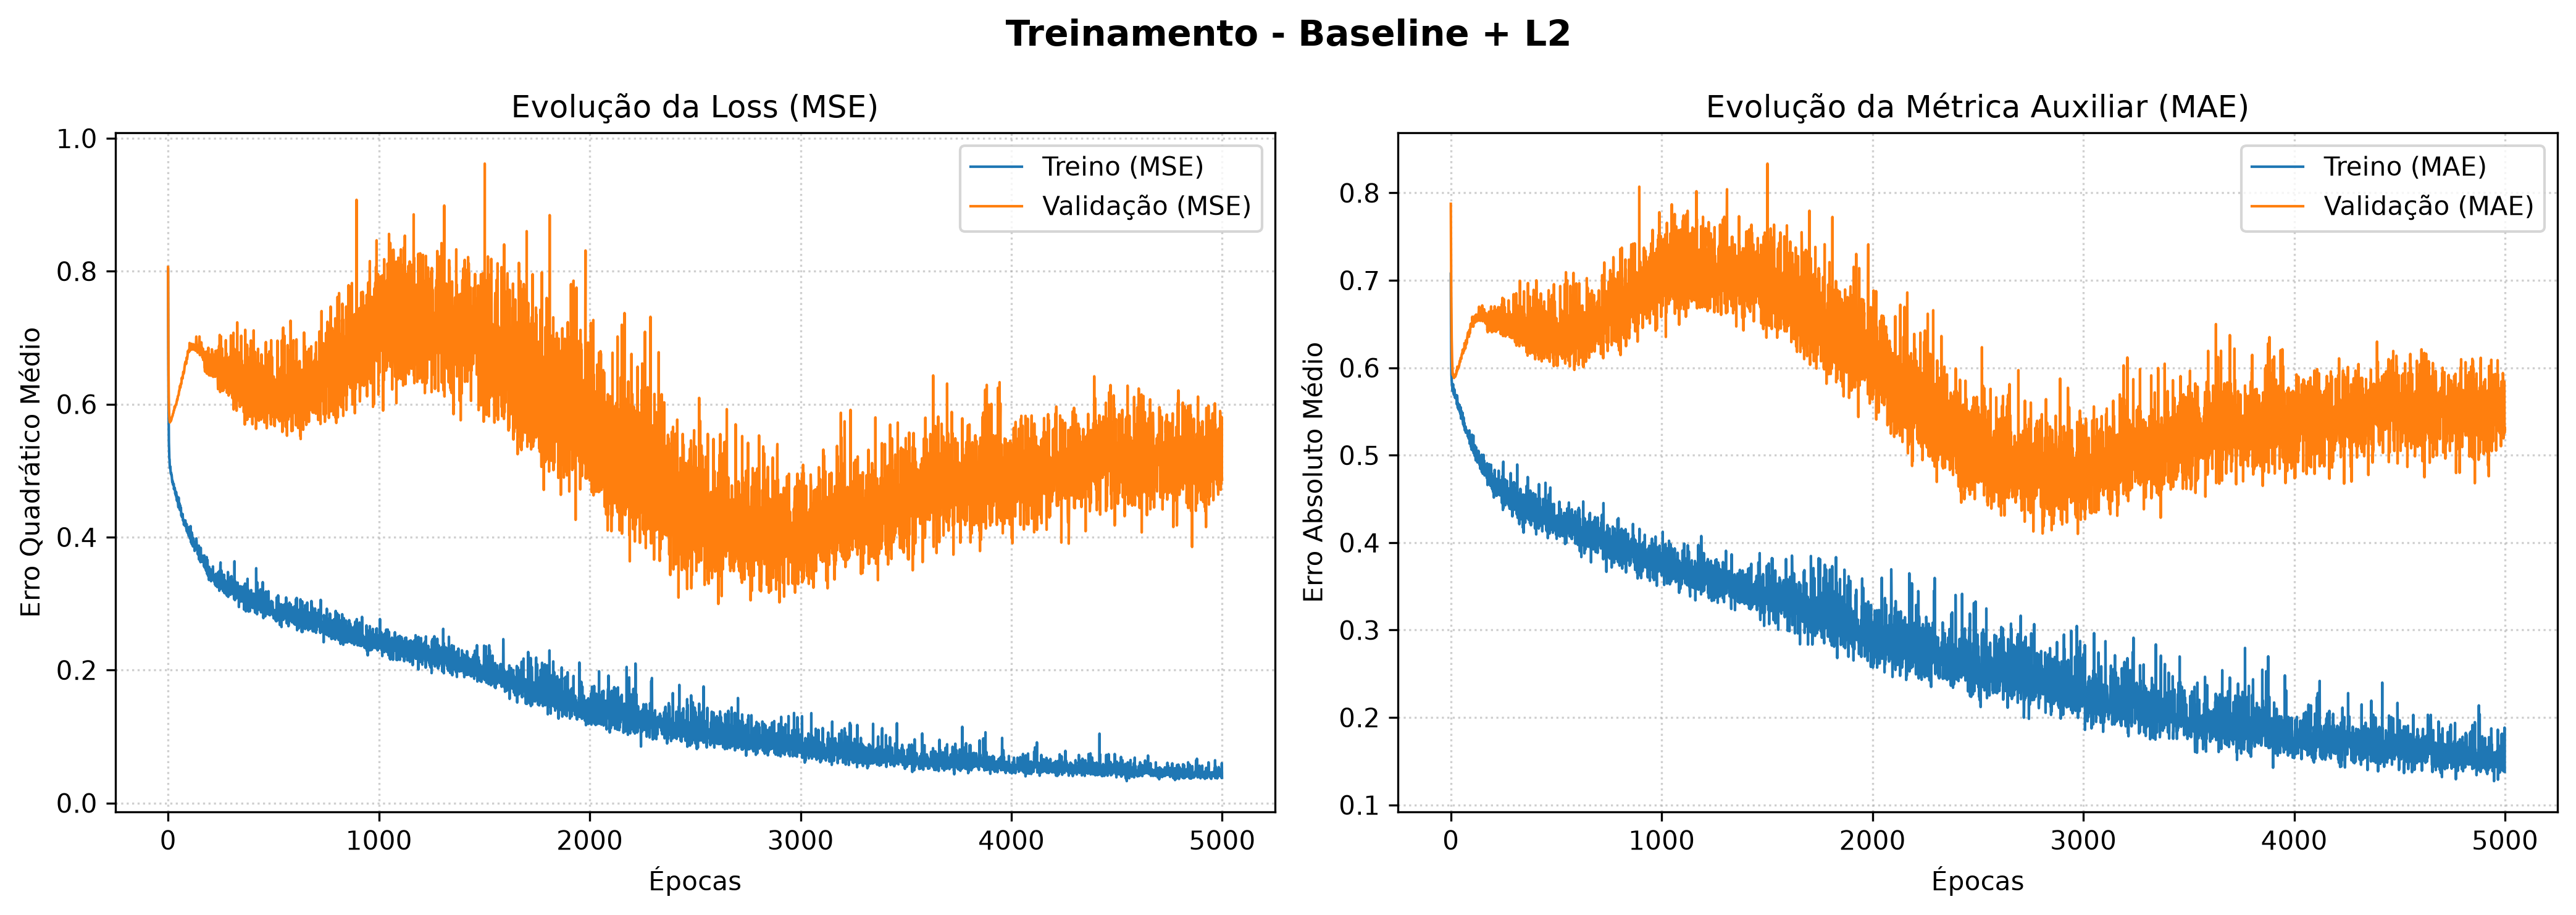
\includegraphics[width=\textwidth]{../src/outputs/baseline_e_l2_history.png}
    \caption{Convergência da MLP Baseline com Regularização L2 ($\lambda = 10^{-6}$).}
    \label{fig:loss_l2}
\end{figure}

\begin{figure}[H]
    \centering
    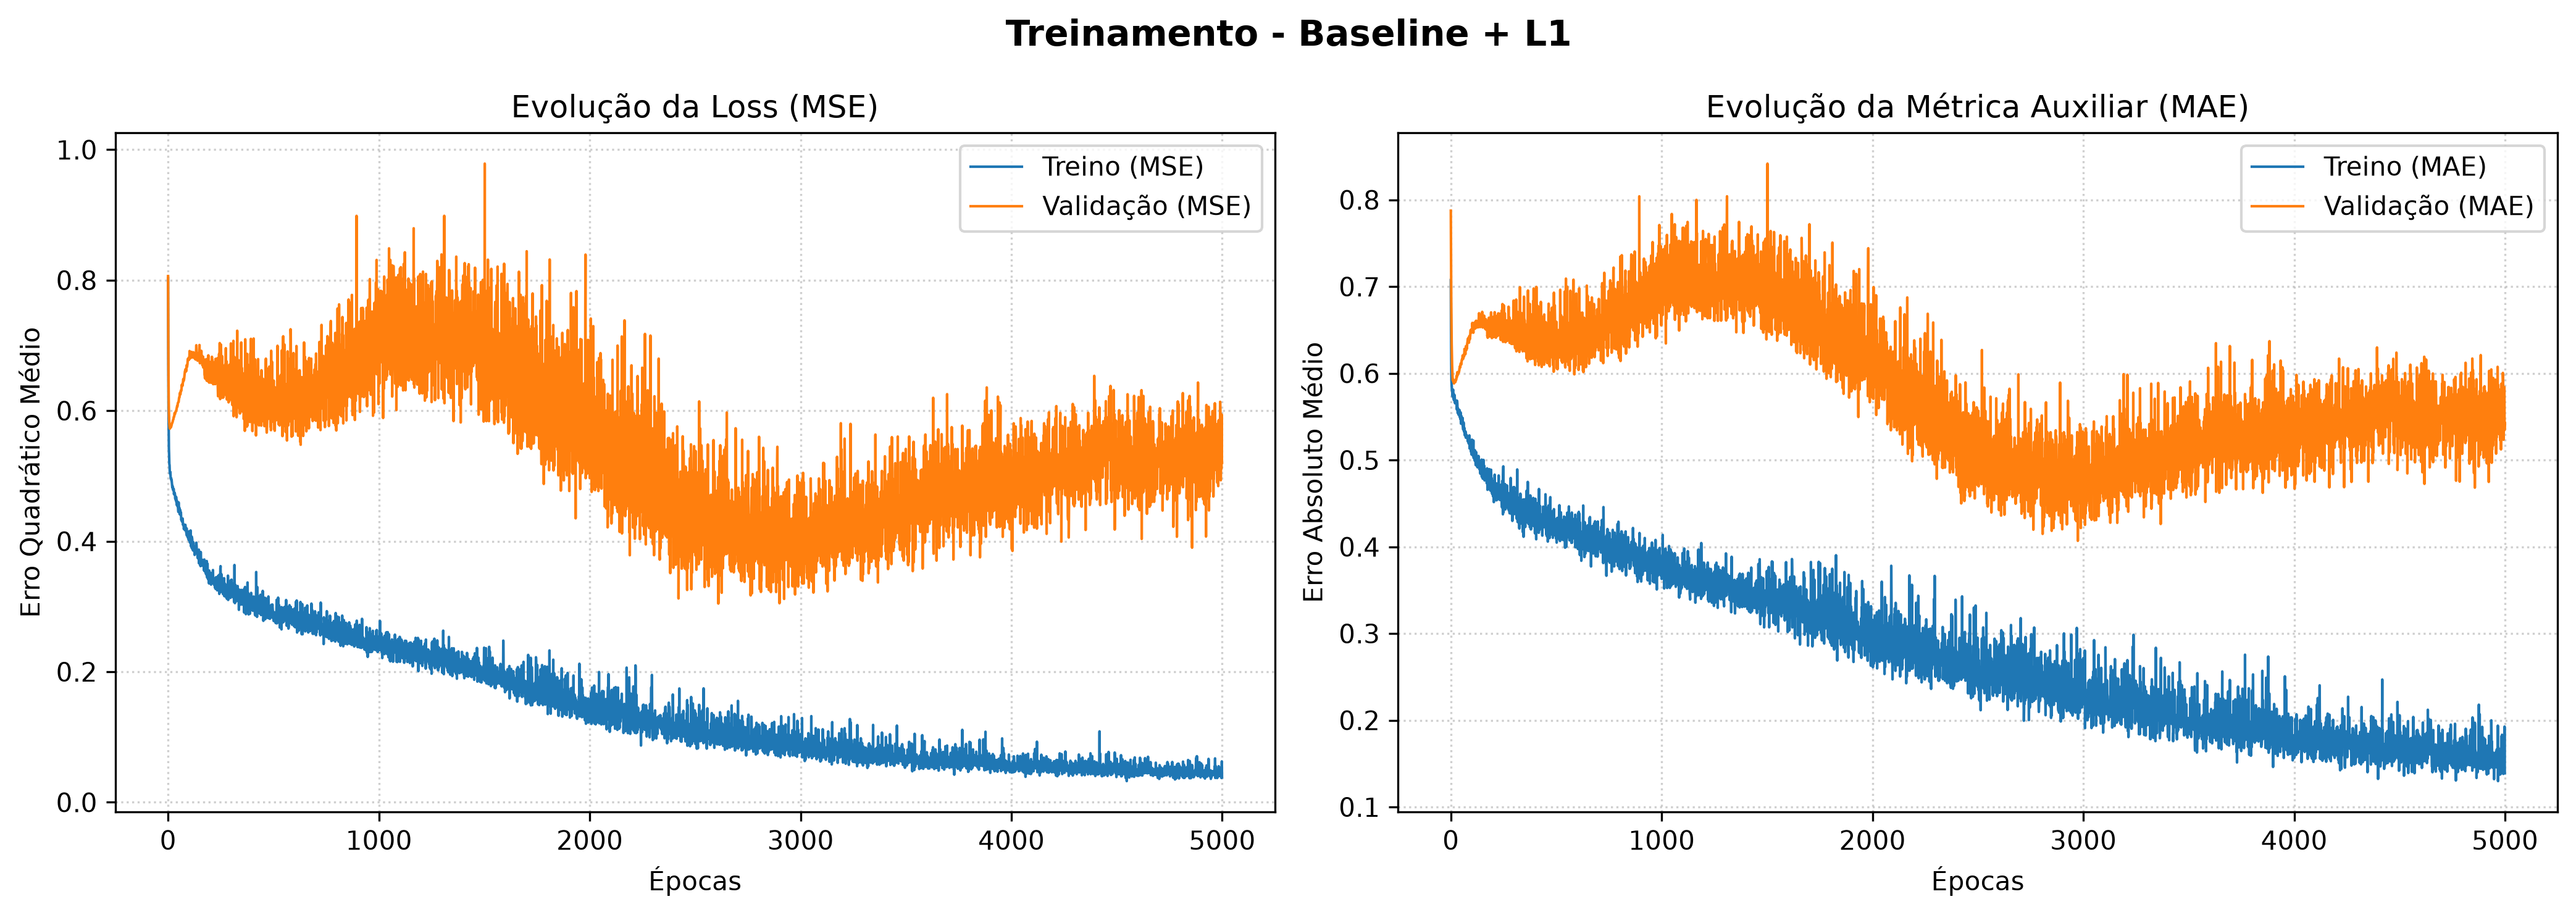
\includegraphics[width=\textwidth]{../src/outputs/baseline_e_l1_history.png}
    \caption{Convergência da MLP Baseline com Regularização L1 ($\lambda = 10^{-5}$).}
    \label{fig:loss_l1}
\end{figure}

\begin{figure}[H]
    \centering
    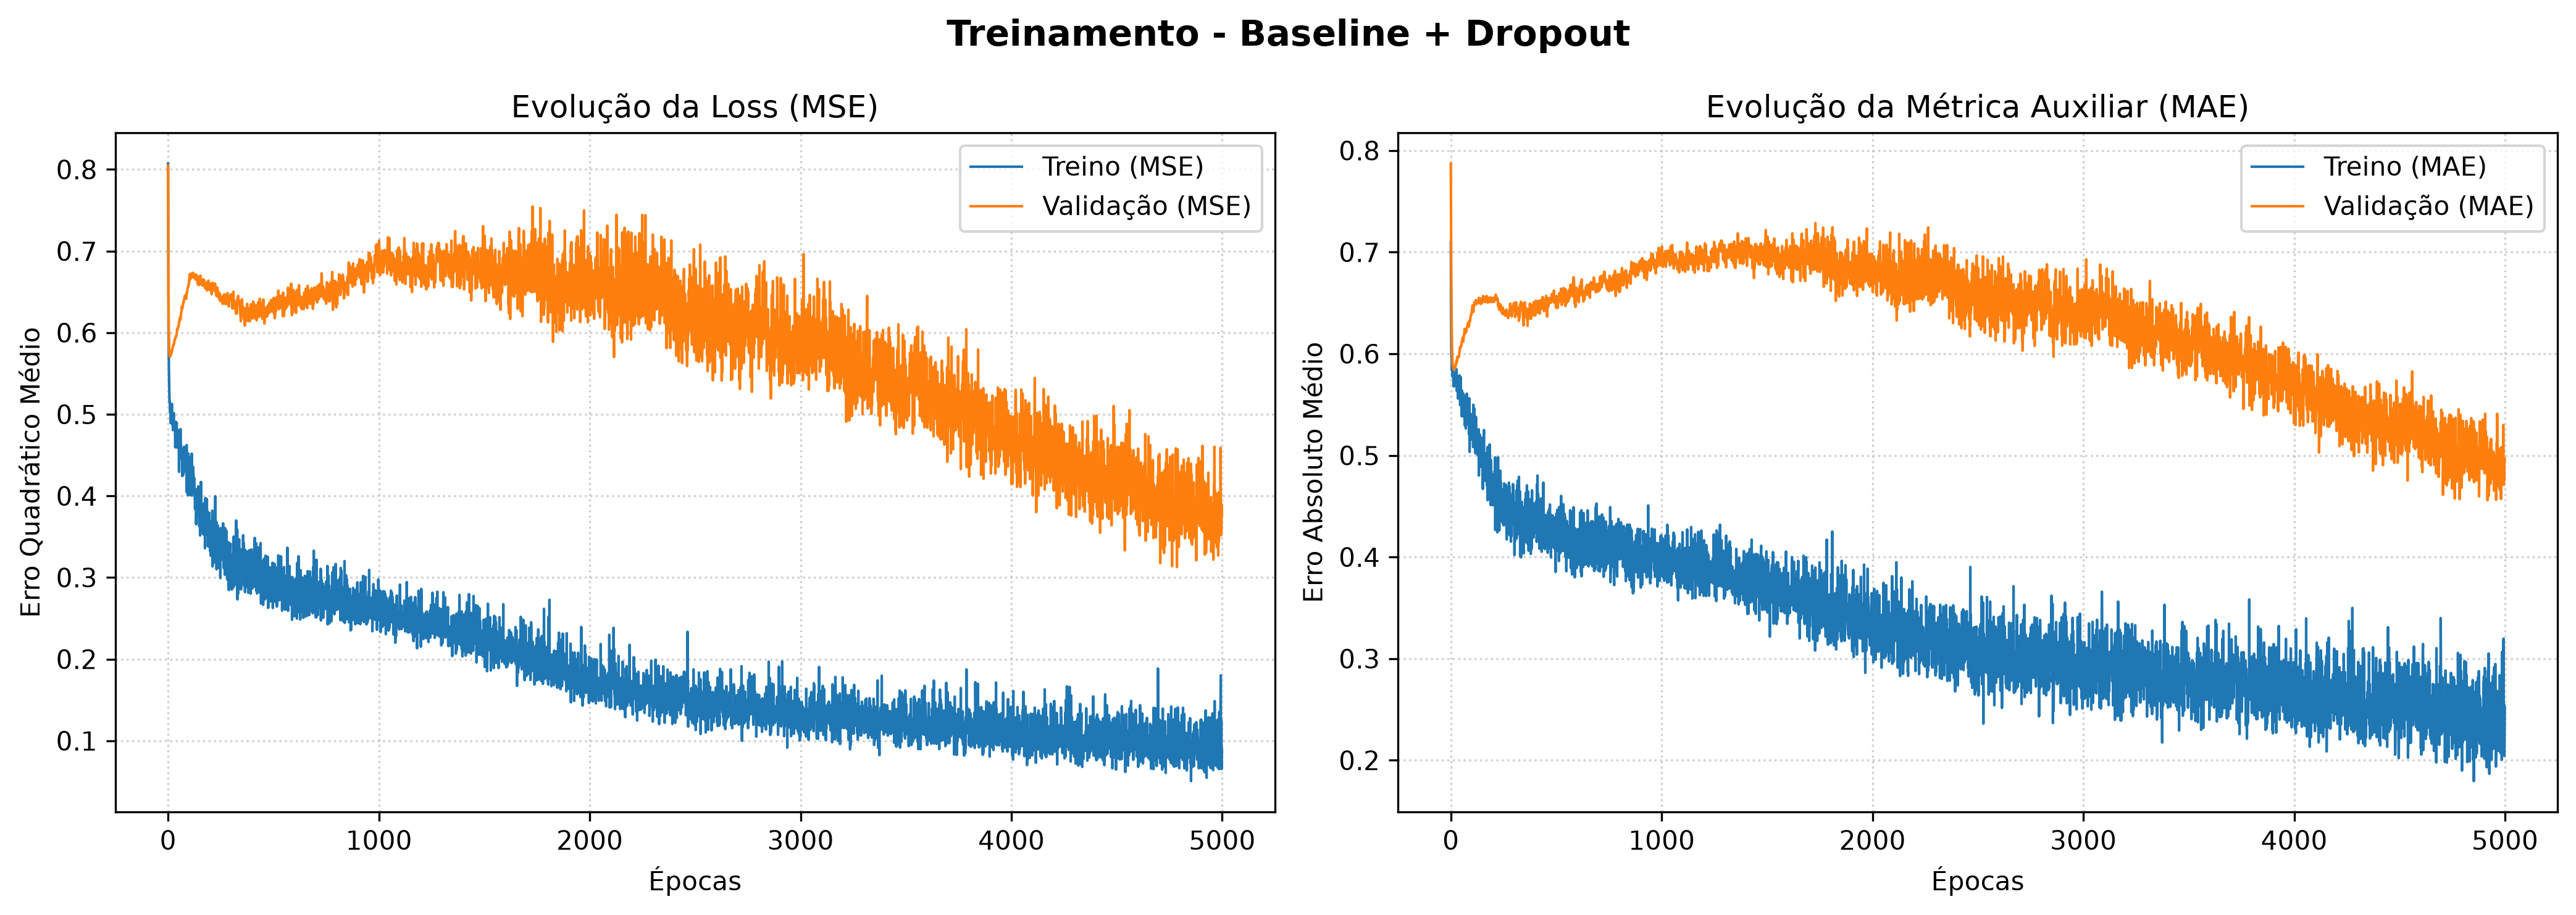
\includegraphics[width=\textwidth]{../src/outputs/baseline_e_dropout_history.png}
    \caption{Convergência da MLP Baseline com Dropout ($p_1=0.1, p_2=0.05$).}
    \label{fig:loss_dropout}
\end{figure}


\subsection{\textbf{Análise Crítica da Dinâmica de Convergência:}}

\subsubsection{Estabilidade do SGD}
Na Figura \ref{fig:loss_baseline}, as perdas de treino e validação apresentam oscilações persistentes. Esse comportamento reflete a limitação do SGD puro com taxa de aprendizado constante: sem reduzir o passo ao se aproximar do mínimo, o modelo sofre contínuo \textit{overshooting}. Além disso, aplicar uma taxa uniforme a todo o espaço de parâmetros gera saltos excessivos nas direções íngremes (causando o ruído) e progresso lento nas regiões suaves. A ausência de mecanismos de suavização, como o \textit{momentum}, faz com que essas instabilidades fiquem evidentes nas curvas ao longo do treinamento."

\subsubsection{Sobreajuste (\emph{Overfitting})}
Na Figura \ref{fig:loss_baseline}, observa-se que os erros de treino e validação se descolaram logo nas primeiras épocas. No decorrer das épocas, observou-se uma intensificação do \textit{overfitting}, visto que o custo de validação passou a crescer e, mesmo com uma queda próxima da época 1500, a curva se estabilizou em uma \textit{loss} muito maior em comparação com o conjunto de treino.

\subsubsection{\textbf{Aceleração com Momentum:}} Na Figura \ref{fig:loss_momentum}, observou-se que a inclusão do momentum reduziu de forma clara o número de épocas necessárias para a \textit{loss} de treino atingir valores baixos. Vale ressaltar que as escalas verticais das Figuras \ref{fig:loss_baseline} e \ref{fig:loss_momentum} são distintas, porém, a partir da evolução da MAE, observa-se que com momentum o modelo atingiu uma \textit{loss} de 0.2 em uma época muito anterior a obtida com o SGD padrão. Essa aceleração ocorre porque o momentum acumula a direção dos gradientes anteriores, de modo que, nas direções em que o gradiente é consistente, os passos se somam e a taxa de aprendizado efetiva aumenta. Em contrapartida, a mesma velocidade acumulada dificulta a "frenagem" dos pesos, que passam do ponto ideal, o que se manifesta como picos abruptos de erro, sobretudo na validação, com valores de MSE de 2 a 4, bem acima do máximo observado no baseline.

\section{Estudo de Ablação e Desempenho no Conjunto de Teste}

Para isolar rigorosamente o efeito de cada componente, a arquitetura base (camadas, ativações e sementes) foi mantida idêntica à da Tabela~\ref{tab:baseline_hiper}, avaliando-se as seguintes variações individuais:
\begin{enumerate}
    \item \textbf{Baseline + Momentum:} SGD com fator de momentum de $\beta = 0.9$.
    \item \textbf{Baseline + Regularização L2 (Weight Decay):} Penalização quadrática dos pesos, com $\lambda_{\text{L2}} = 10^{-6}$.
    \item \textbf{Baseline + Regularização L1 (Lasso):} Penalização por norma $L_1$ para incentivo à esparsidade, com $\lambda_{\text{L1}} = 10^{-5}$.
    \item \textbf{Baseline + Dropout:} Desativação aleatória de neurônios em ambas as camadas ocultas, com ${p_1 = 0.05}$ e  $p_2 = 0.1$.
    \item \textbf{Modelo Combinado:} Baseline + Momentum ($\beta = 0.9$) + Regularização L2 ($\lambda_{\text{L2}} = 10^{-6}$).
\end{enumerate}


\subsection{Análise no Conjunto de Desenvolvimento (Treino e Validação)}

A seleção dos hiperparâmetros e do melhor ponto de treinamento foi realizada com base no menor erro quadrático médio (MSE) observado no conjunto de validação, correspondente a 10\% dos dados. Embora o treinamento tenha sido executado por 5000 épocas, os pesos correspondentes à época de menor MSE de validação foram armazenados e posteriormente utilizados na avaliação do conjunto de teste. Esse procedimento corresponde à seleção do melhor \textit{checkpoint}, não a uma interrupção antecipada do treinamento.

A Tabela~\ref{tab:ablation_train_val} sumariza o comportamento de convergência e os erros de ajuste de cada configuração.

\begin{table}[H]
\centering
\small
\caption{Resultados do Estudo de Ablação: convergência nos conjuntos de treino e validação.}
\label{tab:ablation_train_val}

\begin{tabularx}{\textwidth}{
    >{\raggedright\arraybackslash}X
    c
    c
    c
    c
    c
}

\toprule

\textbf{Modelo / Variação}
&
\textbf{Época Ideal}
&
\textbf{MSE (Tr)}
&
\textbf{MSE (Val)}
&
\textbf{MAE (Tr)}
&
\textbf{MAE (Val)}
\\

\midrule

Baseline Vanilla (SGD)
& 2422
& 0.1007
& 0.3046
& 0.2444
& 0.4420
\\

\addlinespace

Baseline + Momentum ($\beta = 0.9$)
& 2705
& 0.0777
& 0.2422
& 0.2138
& 0.3960
\\

\addlinespace

Baseline + Reg. L1 ($\lambda = 10^{-5}$)
& 2611
& 0.1227
& 0.3045
& 0.2843
& 0.4359
\\

\addlinespace

Baseline + Reg. L2 ($\lambda = 10^{-6}$)
& 2611
& 0.1231
& 0.2994
& 0.2828
& 0.4310
\\

\addlinespace

Baseline + Dropout ($p_1 = 0.05,\ p_2 = 0.1$)
& 4786
& 0.1191
& 0.3128
& 0.2747
& 0.4568
\\

\addlinespace

\textbf{Modelo Combinado}
& \textbf{3215}
& \textbf{0.0499}
& \textbf{0.2869}
& \textbf{0.1730}
& \textbf{0.4359}
\\

\bottomrule

\end{tabularx}
\end{table}


A análise empírica da etapa de desenvolvimento demonstra que o maior ganho observado esteve associado a introdução isolada do \textit{Momentum}, que apresentou o menor MAE de validação (0.3960), superando o \textit{baseline}. A respeitos das regularizações L1 e L2, elas resultaram em um diminuição mínima da \textit{loss} de validação em relação ao \textit{baseline} (0.4420), com MAE de 0.4359 e 0.4310, respectivamente.

As regularizações também produziram aumento moderado do erro de treinamento, comportamento compatível com a restrição imposta à magnitude dos pesos. O \textit{Dropout}, por sua vez, apresentou MAE de validação de 0.4568 e atingiu seu melhor \textit{checkpoint} apenas na época 4786. Esse resultado indica que, para o conjunto de treinamento reduzido utilizado neste experimento, a configuração de \textit{Dropout} adotada não produziu melhora na validação em relação ao \textit{baseline}.

O Modelo Combinado apresentou o menor erro de treinamento (MAE = 0.1730), mas não obteve o menor erro de validação, com MAE de validação de 0.4359.

\subsection{Desempenho de Generalização (Conjunto de Teste)}

A avaliação definitiva da capacidade de generalização dos modelos foi realizada sobre os 80\% dos dados correspondentes ao conjunto de teste (240 amostras). Esses dados permaneceram estritamente isolados e não influenciaram o ajuste dos pesos ou a seleção dos \textit{checkpoints}. Os resultados finais são apresentados na Tabela~\ref{tab:ablation_test}.

\begin{table}[H]
\centering
\small
\caption{Desempenho final no conjunto de teste isolado (80\% dos dados).}
\label{tab:ablation_test}

\begin{tabularx}{\textwidth}{
    >{\raggedright\arraybackslash}X
    c
    c
    c
}

\toprule

\textbf{Modelo / Variação}
&
\textbf{MSE}
&
\textbf{RMSE}
&
\textbf{MAE}
\\

\midrule

Baseline Vanilla (SGD)
& 0.5183
& 0.7199
& 0.5650
\\

\addlinespace

Baseline + Momentum ($\beta = 0.9$)
& 0.4359
& 0.6602
& 0.5189
\\

\addlinespace

Baseline + Reg. L1 ($\lambda = 10^{-5}$)
& 0.5316
& 0.7291
& 0.5715
\\

\addlinespace

Baseline + Reg. L2 ($\lambda = 10^{-6}$)
& 0.5295
& 0.7277
& 0.5691
\\

\addlinespace

Baseline + Dropout ($p_1 = 0.05,\ p_2 = 0.1$)
& 0.4623
& 0.6799
& 0.5280
\\

\addlinespace

\textbf{Modelo Combinado}
& \textbf{0.4248}
& \textbf{0.6517}
& \textbf{0.5131}
\\

\bottomrule

\end{tabularx}
\end{table}


Os resultados do conjunto de teste apresentam um comportamento parcialmente diferente daquele observado na validação. O Modelo Combinado apresentou o menor MAE no conjunto de teste (0.5131), seguido pelo modelo com \textit{Momentum} (0.5189). O \textit{Dropout} também apresentou desempenho inferior ao \textit{Momentum}, mas superior aos modelos com L1 e L2 isoladamente.

Os modelos com L1 e L2 apresentaram MAE de teste ligeiramente superiores ao \textit{baseline}, com valores de 0.5715 e 0.5691, respectivamente. Assim, com os parâmetros utilizados neste experimento, essas duas técnicas não produziram uma melhoria mensurável na generalização.

O \textit{Momentum} apresentou uma redução do MSE de teste de aproximadamente 15,9\% em relação ao \textit{baseline}, enquanto o Modelo Combinado apresentou uma redução de aproximadamente 18,0\%. Esses resultados indicam que, para a configuração experimental adotada, a alteração na dinâmica de otimização teve impacto mais evidente do que as regularizações L1 e L2 isoladas.

Por fim, avalia-se nas Figuras \ref{fig:eval_baseline} e \ref{fig:eval_combined} os gráficos de paridade e de distribuição dos resíduos para os Modelos Baseline e Combinado.

\begin{figure}[H]
    \centering
    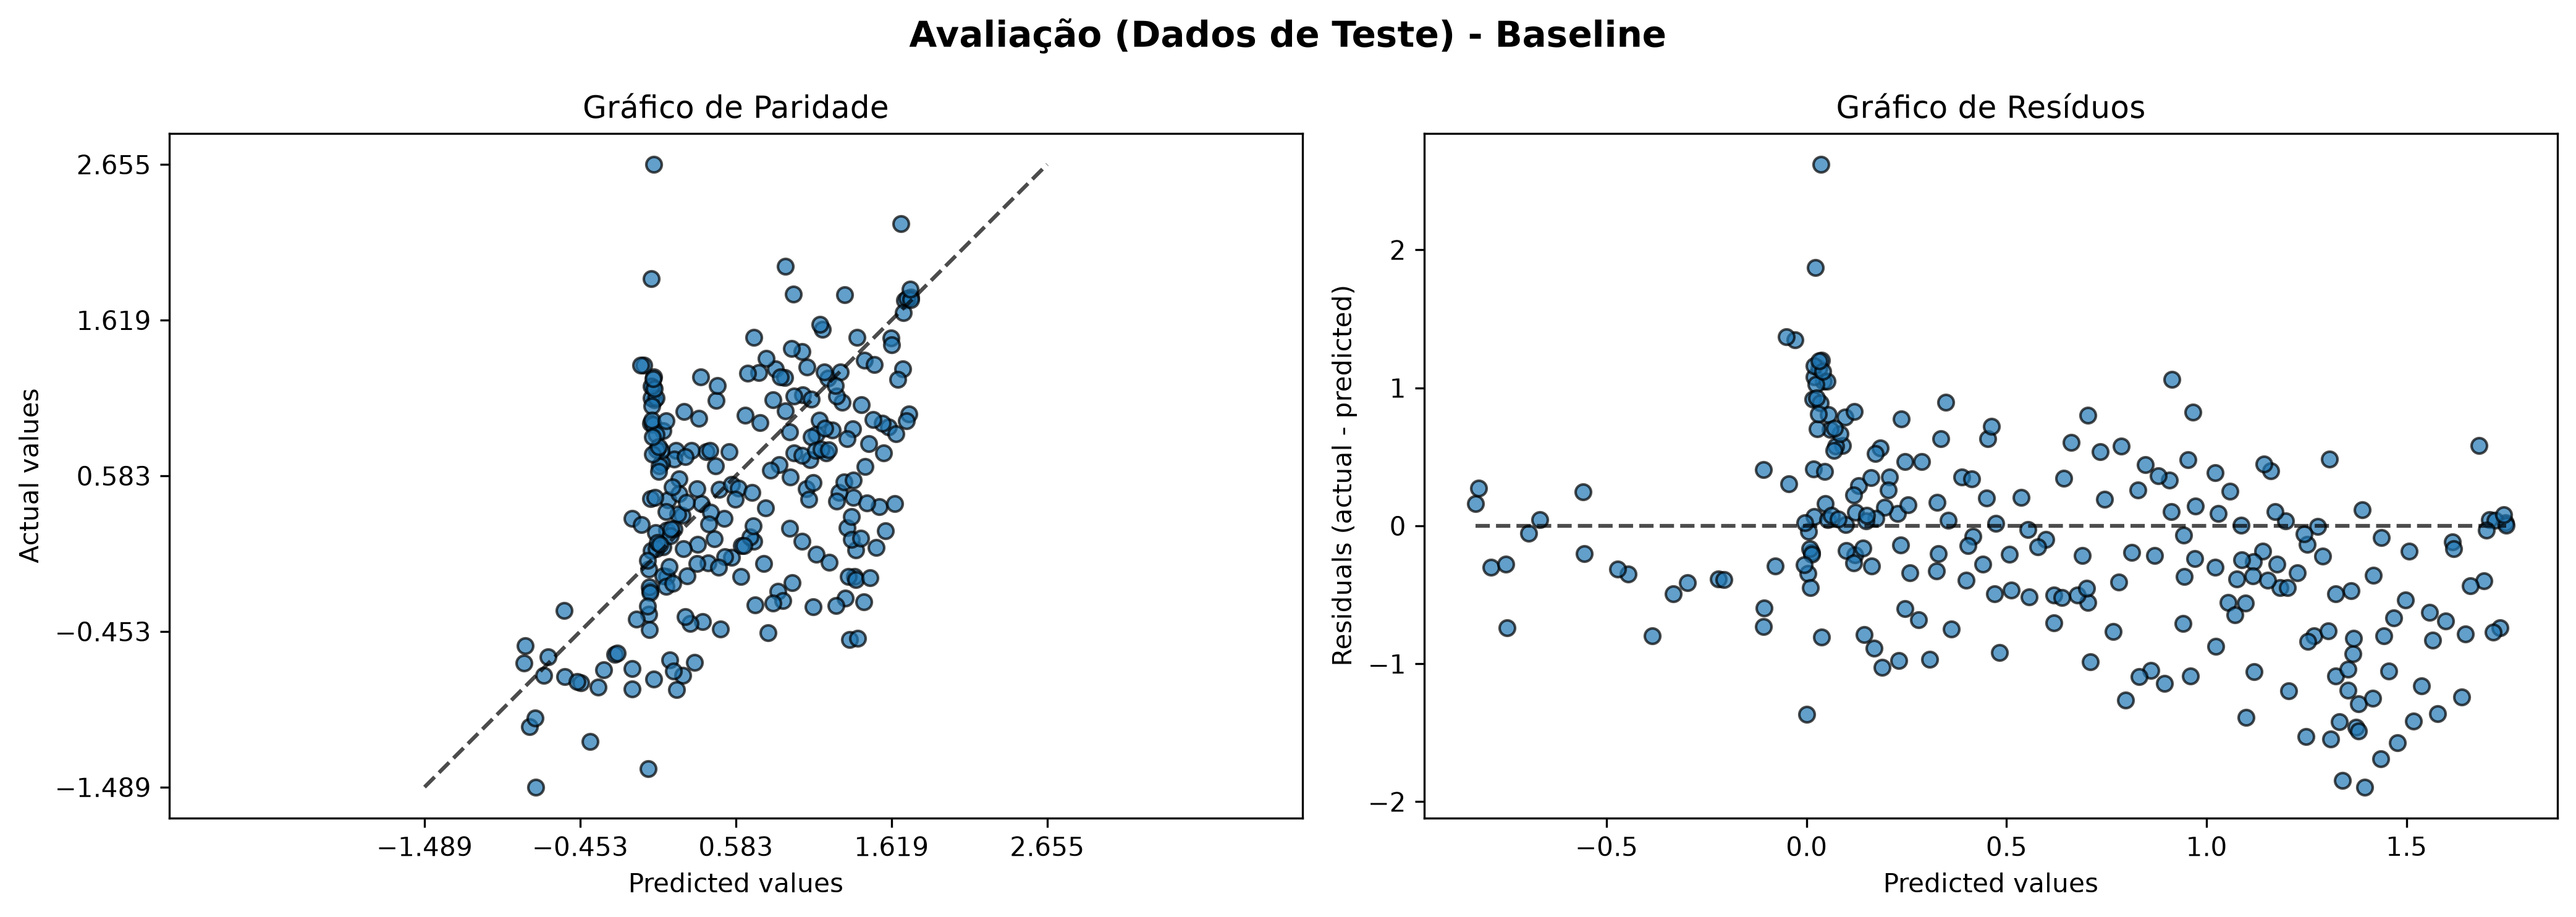
\includegraphics[width=\textwidth]{../src/outputs/baseline_evaluation.png}
    \caption{Avaliação no teste (Modelo Baseline): Gráfico de Paridade e Distribuição de Resíduos.}
    \label{fig:eval_baseline}
\end{figure}

\begin{figure}[H]
    \centering
    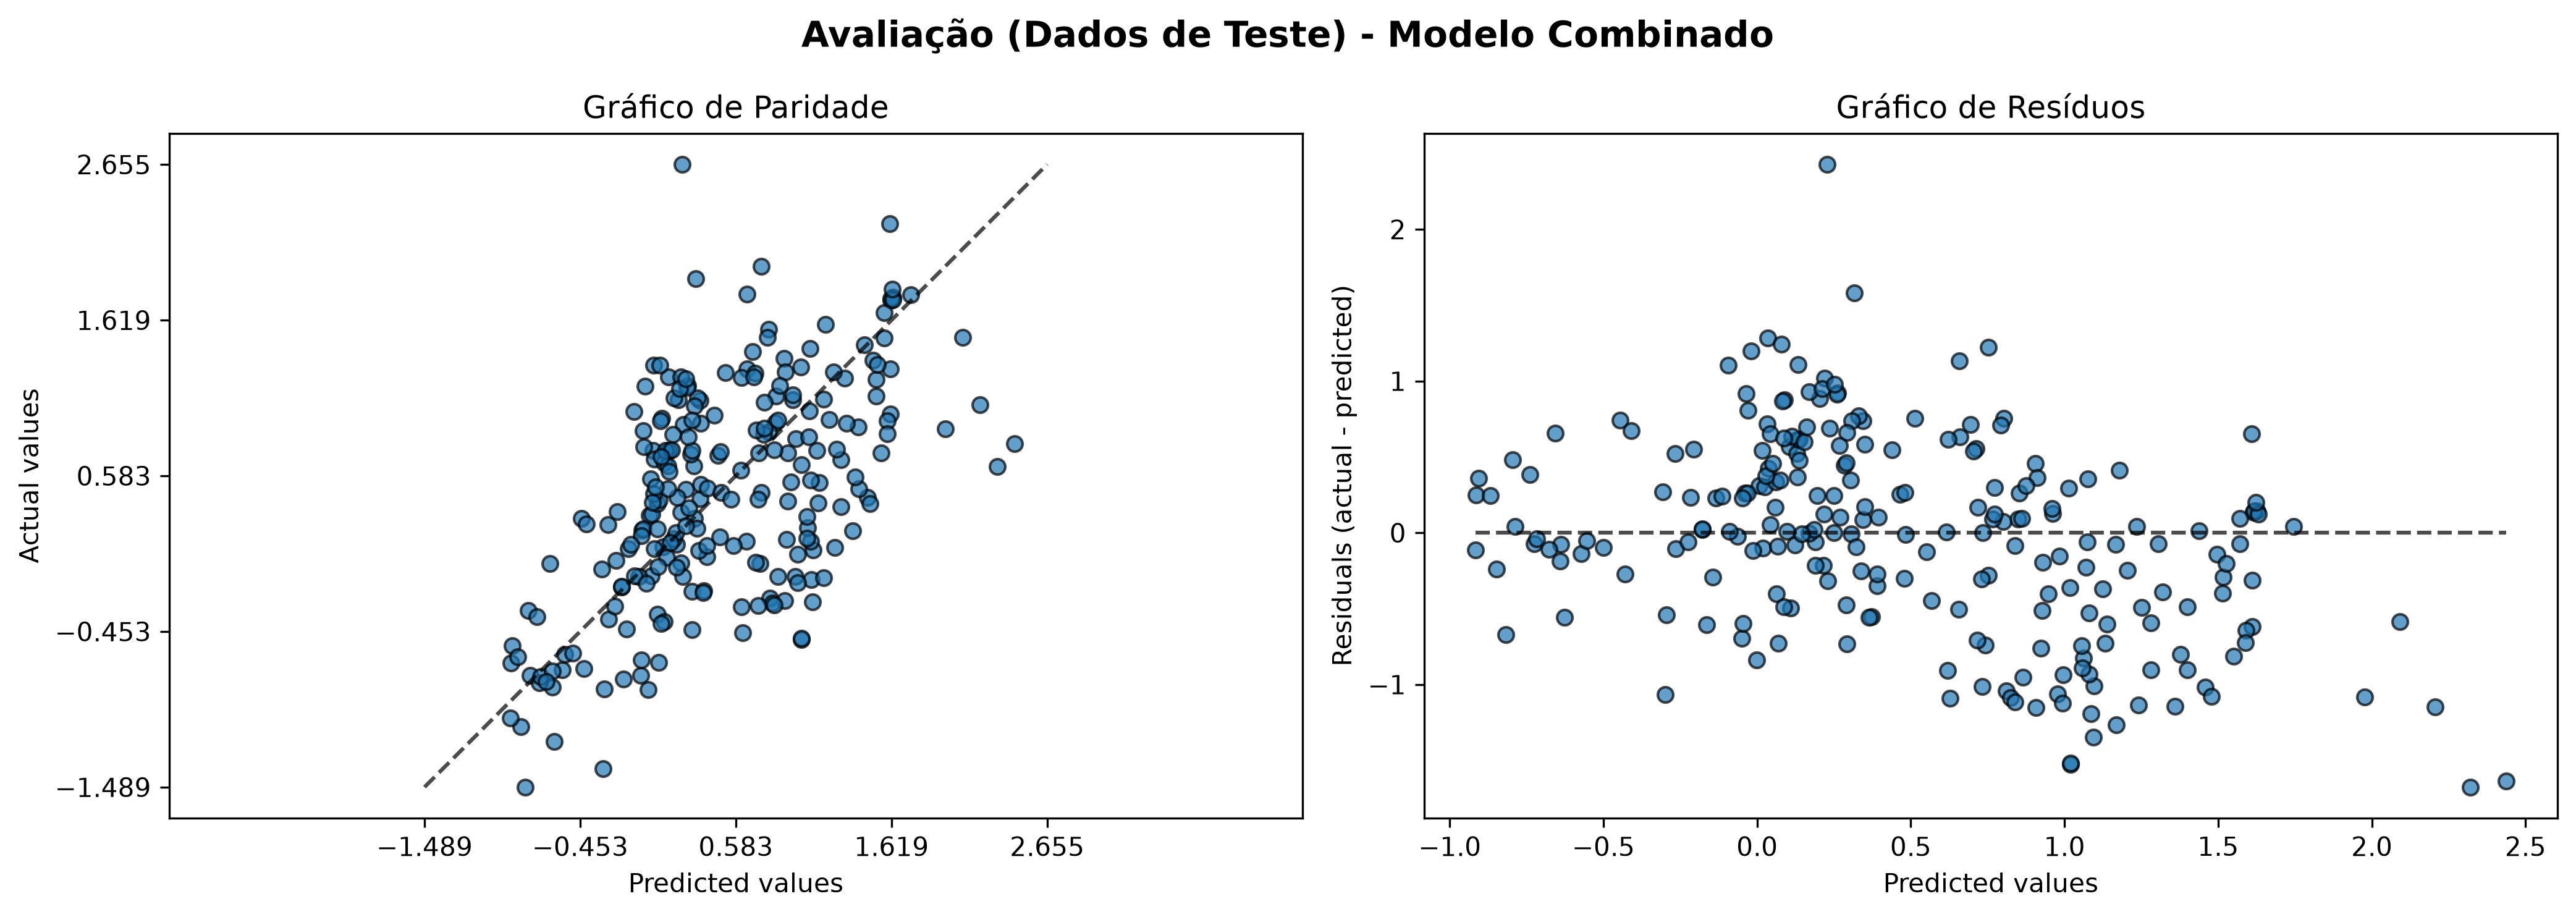
\includegraphics[width=\textwidth]{../src/outputs/modelo_combinado_evaluation.png}
    \caption{Avaliação no teste (Modelo Combinado): Gráfico de Paridade e Distribuição de Resíduos.}
    \label{fig:eval_combined}
\end{figure}

Em ambas as figuras, observa-se que o \textit{baseline} e o modelo combinado compartilham o mesmo padrão geral de erro, embora não sejam idênticos. Em ambos, os resíduos não se distribuem de forma aleatória em torno de zero, sendo eles majoritariamente positivos quando o modelo prevê valores baixos e majoritariamente negativos quando prevê valores altos, isto é, o modelo tende a subestimar no primeiro caso e a superestimar no segundo.

As diferenças entre os modelos aparecem na distribuição das predições. No \textit{baseline} (Figura \ref{fig:eval_baseline}), um grande número de amostras recebe predições praticamente idênticas, embora seus valores reais sejam muito diferentes entre si, e as predições ficam restritas a uma faixa mais estreita. O modelo combinado (Figura \ref{fig:eval_combined}) espalha melhor as predições ao longo de uma faixa mais ampla e apresenta essa concentração de forma menos acentuada, o que é compatível com seu menor MSE de teste na Tabela~\ref{tab:ablation_test}. Ainda assim, a tendência dos resíduos com o valor predito permanece nos dois modelos. Uma explicação plausível é a escassez de exemplos nas regiões extremas do alvo, dado que o treinamento usou apenas 30 amostras.

\section{Discussão e Lições Aprendidas}

\subsection{Impacto do SGD Vanilla no Regime de Poucos Dados (10\% de Treino):}
A arquitetura da rede projetada possui mais de 16.000 parâmetros, um número desproporcional às 30 amostras de treino disponíveis, forçando o modelo a memorizar os dados de treino. O \textit{baseline} reflete esse comportamento com clareza, apresentando um MSE de teste (0.5183) cerca de cinco vezes superior ao de treino. A principal lição extraída desse cenário de extrema escassez de dados é que as regularizações são necessárias para simplificar o modelo, de modo a ser mais generalizável a um novo conjunto do domínio. 

\subsection{Ação Específica dos Hiperparâmetros de Ablação}

A inclusão do \textit{momentum} acelerou a descida inicial da curva de perda, mas inseriu fortes picos de instabilidade, chegando a registrar um MSE entre 2 e 4 na validação. Embora não tenha antecipado a época de convergência ideal (menor \emph{loss} de validação), obteve o maior ganho isolado do experimento, reduzindo o MSE de teste em 15,9\%.

Ao contrapor L1 e L2, neste experimento, observou-se um desempenho virtualmente idêntico, com ambos convergindo exatamente na época 2611 e gerando métricas de teste quase idênticas. Conceitualmente, a regularização L1 costuma se destacar em cenários de alta dimensionalidade por realizar seleção de atributos (zerando pesos de variáveis irrelevantes), enquanto a L2 é indicada para penalizar pesos excessivamente grandes, suavizando as predições do modelo. 

O fato de ambas não apresentarem ganhos substanciais levanta algumas hipóteses atreladas à estrutura do problema: é possível que a L1 não tenha surtido efeito prático porque a rede possui apenas uma dimensão de entrada, não havendo múltiplas \textit{features} para serem selecionadas ou descartadas; já em relação à L2, uma possibilidade plausível é que a extrema superparametrização permita que a rede memorize os dados distribuindo o aprendizado entre milhares de pesos de magnitude muito baixa. Caso isso ocorra, o modelo conseguiria sobreajustar sem necessariamente inflar pesos individuais, o que tornaria a penalização da L2 ineficaz para frear a memorização.

O \textit{dropout}, por sua vez, demonstrou empiricamente seu papel de regularização. Observou-se que houve uma diminuição na métrica de treino (com aumento de 18\% no MSE) e um atraso substancial na convergência (alcançando o valor ótimo apenas na época 4786). Assim, a lição extraída é que simplificar a representação inicial do treinamento pode ajudar a rede a mapear características mais genéricas, garantindo um desempenho superior frente a dados inéditos.

Por fim, o Modelo Combinado fornece uma lição clara sobre a sobreposição de hiperparâmetros. Observou-se que os ganhos não são simplesmente aditivos. O \textit{momentum} isolado foi responsável pela maior melhoria do experimento (queda de $\sim$16\% no MSE de teste). A L2, isolada, não apresentou ganhos reais sobre o \textit{baseline}. Quando unidos, o Modelo Combinado obteve menores \emph{losses}, mas obteve um ganho apenas marginal sobre o modelo contendo apenas \textit{momentum}.

\subsection{Análise de Resíduos e Limitações Estruturais}
Como evidenciado na seção anterior, a análise visual confirmou que o modelo regularizado não superou as falhas estruturais nas caudas da distribuição. O padrão de superestimar valores muito negativos e subestimar valores altos persistiu de forma inalterada em ambas as abordagens. 

A principal lição extraída é que esse viés não reflete um ajuste ruim de hiperparâmetros, mas sim um sintoma direto da escassez de dados. Com apenas 30 amostras de treino, a rede carece de representatividade nas extremidades do problema e acaba concentrando suas previsões em torno da média local. Fica demonstrado, portanto, que as técnicas de regularização podem ser eficazes para reduzir a magnitude do erro absoluto, mas não conseguem suprir a ausência de informação estrutural nem corrigir vieses derivados de amostragem insuficiente.

\end{document}
